

\section{Data Collection Process}
In this section more details on how data was collected from each system will be presented. 

\subsection{MicroPilot AutoPilot}
\subsubsection{Instrumentation}
Control decisions in this software are made in a 5Hz loop, it means that every 200ms all the sensor inputs are read and based on the current state of the aircraft and the system's goal at the moment (e.g. maintaining a constant speed) decisions will be made and output is generated. Considering this, the best way to capture those data is in the end of each iteration of this loop. I inserted instrumentation code there, to log input and output values (listed in Table~\ref{tab:in_outs}) at the exact spot where they are updated. 
Please note that although it is more convenient to capture the values in this way, it does not give us any special advantage or insight that breaks the black-box condition. In other words, the exact same data could be collected from the compiled binaries without any access to the internals, just with extra steps. Inputs and outputs, after all, are the very least thing available in both black-box and white-box settings.

\subsubsection{Test Scenarios}\label{sec:mp_test_scenarios}
MicroPilot has a repository of 948 system tests, I ran them in a software simulator\footnote{It is developed by MicroPilot and provides an accurate simulation of the aerodynamic forces on the aircraft, the physical environment irregularities (e.g. unexpected wind gusts), and noises in sensor readings} and collected the logged flight data, over time. 
The test cases are system-level tests. Each test case includes a flight scenario for various supported aircraft. A flight scenario goes through different phases in a flight such as ``take off'', ``climb'', ``cruise'', ``hitting way points'', and ``landing''.
\begin{table}
    \caption{The $n=10$ collected I/Os of AutoPilot. The inputs are sensor readings and the outputs are the servo position update commands. All these I/Os over time are used as the inputs of the state prediction model.}
    \label{tab:in_outs}
    \centering
\begin{tabularx}{\columnwidth}{lX}
                                                                                                                    \toprule
\multicolumn{2}{l}{\textbf{Inputs}}                                                                              \\ \midrule
Pitch     & The angle that aircraft's nose makes with the horizon around lateral axis                            \\ 
Roll      & The angle of aircraft's wings make with the horizon around longitudinal axis                         \\ 
Yaw       & The rotation angle of aircraft around the vertical axis                                              \\ 
Altitude  & AGL\footnotemark Altitude                                                                            \\ 
Air speed & Speed of the aircraft relative to the air                                                            \\ \midrule
\multicolumn{2}{l}{\textbf{Outputs}}                                                                             \\ \midrule
Elevator  & Control surfaces that control the Pitch                                                              \\ 
Aileron   & Control surfaces that control the Roll                                                               \\ 
Rudder    & Control surface that controls the Yaw                                                                \\ 
Throttle  & Controller of engine's power, ranges from 0 to 1                                                     \\ 
Flaps     & Surfaces of back of the wings that provide extra lift at low speeds, usually used during the landing \\ \bottomrule
\end{tabularx}
\end{table}
\footnotetext{Above Ground Level}
Out of the 948 flight logs, I omitted 60 that were either too short or too long (shorter than 200 samples or longer than 20k samples). Figure~\ref{fig:test_lengths} shows the distribution of the remaining log lengths. The maximum length ($L$) was 18,000 samples.

\begin{figure}
    \centering
    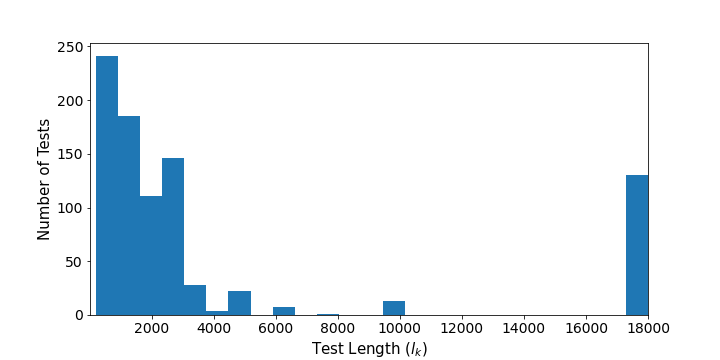
\includegraphics[width=\columnwidth]{ASE_files/test_lengths.png}
    % \Description[Number of tests histogram]{A histogram chart maxing on numbers less than 2,000 and over 17,500}
    \caption{Distribution of flight log lengths for the $N=888$ (out of the original 948 available logs) logs that were kept in the dataset ($200 \leq l_k \leq 20,000$), \hl{from MicroPilot.}}
    \label{fig:test_lengths}
\end{figure}

% As mentioned before each input data item is a multivariate time series with $n=10$ variables (listed in table~\ref{tab:in_outs}). 
% During the data preprocessing, after the time series data is converted into tensors, all of the shorter $T_i$s were post-padded to the length of the longest one: $L=18000$ time steps.
The dataset was randomly split into three chunks of 90\%, 5\%, and 5\% for training, validation, and testing, where each sample corresponds to one test execution. Note that separate test and validation sets are needed to facilitate proper hyper-parameters tuning, without leaking information. 
% \subsection{System Under Study} \label{mp_data_collection}
% Our case study is a state-based system, which is real-time controller for UAVs, developed by
% our partner
% \begin{anonsuppress}
% Winnipeg based Micropilot Inc. Micropilot is the world-leader in professional UAV AutoPilot which develops both hardware and software for 1000+ clients (including NASA, Raytheon, and Northrop Grumman) in 85+ countries during the past 20+ years.
% \end{anonsuppress}
% .

%What the AutoPilot does can be summarized as `trying to hold some invariants based on the goal/state of the system'.
% % Maybe these two paragraphs can be moved somewhere more appropriate
% \label{changes_in_inputs}
% To work it backwards we capture the input/outputs (the UAV's relevant signals) over time and examine their correlations, i.e. how changes in one of them results in changes in another. When the state of the system changes these relations may change. So if we can capture what the relations are and when they change we can determine the state in which the system is in. 
% Of course pinpointing the exact moment when the changes happen is difficult; It is also impacted by the sampling time resolution so the inferred states and the change points are approximations.
The auto pilot can be used in SWIL and HWIL modes \cite{melmoth2019true}, which stand for software in the loop and hardware in the loop respectively. I used SWIL mode as it provides what was needed without any of the costs and hassles that come from HWIL mode. 

\subsection{Paparazzi}\label{sec:paparazzi_data_collection}

\hl{This sub section is new}

\subsubsection{Instrumentation}
Paparazzi provides a rich and flexible API that can be configured to record several different parameters in flight. The aircraft periodically sends data back to the ground station over a wireless link using a protocol called Paparazzi link. Paparazzi link is built over Ivy, a message bus protocol that uses UDP. 
In Paparazzi's architecture a process called `link' interfaces the wireless link to the aircraft to the computer's network; on one side are the Paparazzi link messages that come and go as UDP datagrams and on its other side is the (often wireless\footnote{A wired connection is used in HWIL test mode as well as some scenarios where the AutoPilot equipment is used in a autonomous submarine rather than an autonomous unmanned aircraft.}) connection to the aircraft.
In simulations, the modem and wireless communications are no longer needed, instead the auto pilot runs as a separate process and mimics a wireless channel over the local network. (See Figure~\ref{fig:paparazzi_comm_agents})

\begin{figure}
    \centering
    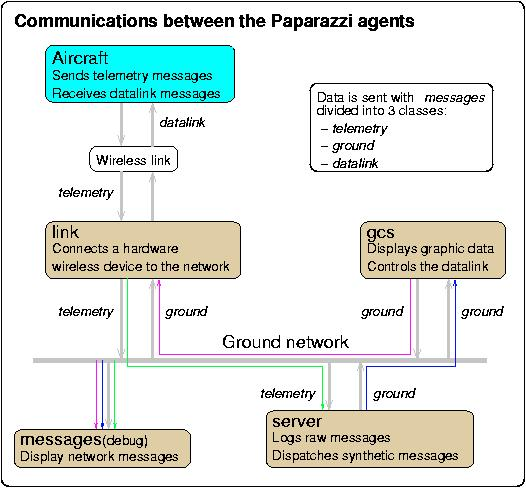
\includegraphics[width=\columnwidth]{4_files/Pprz_communication_agents.jpg}
    \caption{High level overview of communication links architecture in Paparazzi \cite{hattenberger2014using}}
    \label{fig:paparazzi_comm_agents}
\end{figure}

Paparazzi comes with a multitude of small tools that could do most of what I needed in terms of instrumentation. There is a remote logger and a log player which are quite close to the instrumentation tool I need, however upon trying them in action, I figured that they cannot record some of the information that I need. Therefore, I developed a custom flight data recorder tool. 

\subsubsection{Test Scenarios}
Unlike MicroPilot that had a quite a number of system tests (in addition to other types of tests such as unit tests which I did not use), Paparazzi comes with only unit tests. As it is an open source software under GPL licence it comes with no warranty and also does not need certain certifications and approvals that commercial systems require, therefore incentives to have such tests are lower. 
Although it is a reliable and widely used auto pilot, it owes that reliability more to its widespread use in action (by many researchers and enthusiasts) rather than automated tests that verify its behaviour.
In this situation, where many eyes are watching over the code, bugs are discovered and patched quickly. However, to the best of my knowledge they are not recorded as system tests that verify the bugs are properly patched and detect regressions in the future.

To fill the void, I created a fuzz testing tool that can automatically generate valid, diverse, and meaningful automated system tests for Paparazzi based on the example flight plan that is included with it.
My tool can automatically generate system tests, run them in a simulator (or on hardware\footnote{Although I have not tested running tests on a hardware (HWIL) to confirm, but having implemented the protocol it potentially is capable of doing so}), and also collect required telemetry data from the aircraft. 
%run them automatically, and integrated it with the flight data recorder tool to generate the data set for downstream tasks. 
It is called PprzTester and the source code, version history, project planning data (bugs, enhancements, tasks and issues, etc), and the documentations are available on GitHub at \url{https://github.com/MJafarMashhadi/pprz_tester}. 
The targeted randomizations in test inputs are augmented with the stochastic wind model in the simulation to further diversify the observed behaviours.

In addition to that tool, I needed to patch some parts of Paparazzi to make the logging and testing more similar to MicroPilot, for example increase telemetry reporting rate from 2Hz to 5Hz. A list of these patches including the reason why that change was necessary or beneficial and the exact lines of code that need to be changed is available in the project wiki at \url{https://github.com/MJafarMashhadi/pprz_tester/wiki/Paparazzi-Patches}.
Aside from the patches, I found some bugs, missing features, missing documentations, and bad smells in the code that needed to be fixed. I contributed new code and documentation to the Paparazzi project to address these issues. The contributions were useful, up to the standards, and welcome in the project; they are included in the latest release\footnote{as of August 3rd, 2020} of Paparazzi auto pilot: version 5.16.

More details about the tool is left for next section, section~\ref{section:fuzzing_tool}.
The result of generating and running tests was 378 runs worth of different flight scenarios.
After collecting the data I performed some pre-processing steps on them to make them more similar to what the previous model was trained on. These pre-processing steps include normalizing some values as well as metric to imperial unit conversions.

Figure~\ref{fig:paparazzi_test_length} shows the distribution of the test lengths. The test lengths range from 140 samples (70 seconds) to 2580 samples, with a median of 2170 and a mean of 1896.
\begin{figure}
    \centering
    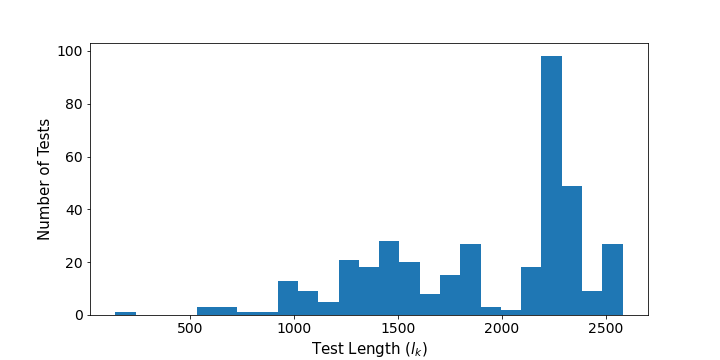
\includegraphics[width=\columnwidth]{6_files/test_lengths.png}
    \caption{The histogram of number of tests of different test sizes. The smallest samples contains 140 samples worth of recorded flight data and the largest one has 2580 samples, equivalent of a 516-second flight (Sampling rate is 5Hz). }
    \label{fig:paparazzi_test_length}
\end{figure}

The training data was split into 3 chunks after shuffling: 70\% of the data was used for training, 20\% was used as the test set for tuning the hyper-parameters, and the remaining 10\% was set aside as the validation data to measure the trained model's performance. 







\subsection{The Testing and Data Processing Tool Set}\label{section:fuzzing_tool}
I implemented the pipeline of generating tests, running them, and aggregating flight logs in an integrated tool with three components, one for each stage. In the following sections I will explain these components and their role in the system. I also very briefly explain how event-driven programming paradigm was implemented here both to decrease coupling and to make it more resilient to unexpected or buggy behaviour. It is necessary for two reasons: 1. as a testing tool, it is \textit{expected} to encounter bugs in software under test and should be resilient to them 2. the message passing design of Paparazzi architecture, in addition to its ability to support multiple aircraft in flight at the same time left me with no choice but to use an event-driven design.


\subsubsection{Flight Data Recorder}
Although Paparazzi comes with a logging feature in its `server' component (Figure~\ref{fig:paparazzi_comm_agents}), it only logs a subset of required data. Furthermore, the data comes in separate messages with different frequencies; for example speed updates are sent in \verb|AIRSPEED| message once a second, orientation updates and engine rpm are reported in \verb|ATTITUDE| and \verb|ENGINE_STATUS| messages respectively which are dispatched every 200 milliseconds, while servo outputs are only sent once every 5 seconds. All these data need to be aggregated and aligned. Please refer to the Table~\ref{tab:pprz_messages} in \hyperref[appendixa]{Appendix~A} for a full list of messages used.

The most flexible option with the least overhead is to have an independent module that understands Paparazzi link, captures these messages and does data aggregation and logging in real-time. So I created a flight data recorder to collect all the required data from telemetry messages.

In the beginning the instance of ``AircraftManager'' singleton class starts with listening for \verb|NEW_AIRCRAFT| messages. This message type notifies this class when new aircraft come online in the simulation. Then it sends a \verb|AIRCRAFTS_REQ| request message to server to get a list of currently online aircraft. The response to both of these messages are processed in the same way: The aircraft unique ID will be checked against the hash table of known aircraft, if it is a new one an ``Aircraft'' instance will be created and added to the hash table. (See the class diagram in Figure~\ref{fig:fdr_class_diagram} in \hyperref[appendixa]{Appendix~A})

Each ``Aircraft'' object in the makes a number of requests back and forth with other components in the system (server, data link, and the auto pilot process) to gather required information about that aircraft, including its flight plan. This class along with ``Aircraft Parameters'' and ``Aircraft Commands'' provide a unified programmatic API for monitoring and controlling the aircraft. 

I implemented observer pattern \cite{gamma1995design} in ``Aircraft Parameters'' to enable other components (such as flight data recorder and automated test executor) to listen for changes in the aircraft state and respond accordingly in an event-driven manner. 
After creation of an ``Aircraft'' object, as a part of its initialization, several observers are created and attached to it. A ``Record Flight'' instance is one of them. It observes new \verb|FLIGHT_PARAM| messages as well as changes in `throttle', `flight time', and `commands.values' parameters. This class stores and aligns these parameters in a pandas data frame which is stored on disk periodically. The data can be stored in a human-readable CSV file or as a compressed HD5 binary. Some data normalization and unit conversions (such as meters to feet) also happen before saving in order to make the generated data similar to MicroPilot's.

Supplementary UML diagrams are provided in \hyperref[appendixa]{Appendix~A}.


\subsubsection{Automated Test Executor}
Here I first explain how the test executor work, since knowing this is prerequisite of understanding the test generator component.
The test executor takes the control of the aircraft by running prefabricated test scenarios. While the low level control of the aircraft is done by the auto-pilot software (the system under test), it needs high level commands such as ``climb to 200ft''. Automated test executor does that, using hand crafted test scenarios or the ones generated by the test generator component.

Tests scenarios are defined as subclasses of \verb|PlanBase| class. Each plan needs to override a method that returns an iterable of plan items which should be executed one by one. 
\begin{lstlisting}[language=Python, basicstyle=\linespread{0.1}]
class ExamplePlan(PlanBase):
  def get_items(self, **kwargs):
    block_name = kwargs.pop('block_name')
    circles = int(kwargs.pop('circles'))
    return [items.JumpToBlock(block_name),
      items.WaitForCircles(n_circles=circles)]
\end{lstlisting}
The above plan for example, takes a block name and a number of circles as its parameter and executes the two items in succession. An example of running this plan can be like the command below:
\begin{lstlisting}[language=bash]
$ run_test.py ExampleAircraft ExamplePlan\ 
    -Dblock_name='loiter' -Dcircles=2
\end{lstlisting}
Using this parameters is analogous to test parameterization in mature unit testing frameworks (such as pytest). It allows similar test plans that are only different in some parameters to be consolidated in one test case.
Using parameters also improves the reproducibility of test scenarios while improving its flexibility. Test scenarios (plans) do not need to include commands for waiting for aircraft to take off and land, the testing tool automatically wraps it with appropriate initialization code.

The core test plan runner is implemented as an observer class that listens for multiple messages and parameters to get notified about changes in the aircraft's state (See Figure~\ref{fig:flight_plan_executor_class_diagram} in \hyperref[appendixa]{Appendix~A}). It iterates over the flight plan items and calls their \verb|match| method to decide whether that item should be executed. Whenever a match is found the item will be executed and the iterator will move to the next test plan item. Consult Figure~\ref{fig:flight_plan_items_class_diagram} in \hyperref[appendixa]{Appendix~A} for a class diagram of all flight plan items.

Test plans should be importable from \verb|pprz_tester.generated_plans| module. The structure is simple and clearly defined so that they can easily be handcrafted (like the example above) or generated using the test generator component.

The test runner is tailored specifically for Paparazzi in several ways:
\begin{enumerate}
    \item % First, 
As mentioned before, it takes care of aircraft initialization, take off, and landing
    \item %Second, 
It uses standard Paparazzi environment variables such as \verb|$PAPARAZZI_HOME|.\footnote{If it is not set, the user can use \texttt{-p /path/to/paprazzi} command line argument to set this value, and if that is not set too, a default value will be used.} 
    \item %Third, 
It can build the auto pilot if \verb|--build| argument is set so the user does not have to build it manually in Paprazzi center. 

    \item %Fourth, 
If \verb|--gcs| argument is set, the ground control station window will be opened (See Figure~\ref{fig:paparazzi_gcs}). It provides a real-time map that visualizes the aircraft path, waypoint locations, wind direction and velocity, and several other parameters of the aircraft such as their airspeed and altitude. 
    \item %And last, 
\verb|--no-sim| argument tells tester to not launch the simulator. Its use case can be when a physical auto pilot is being used (similar to MicroPilot's HWIL mode), or when for any reason the user chooses to run the simulator manually. 
\end{enumerate}

\begin{figure}
    \centering
    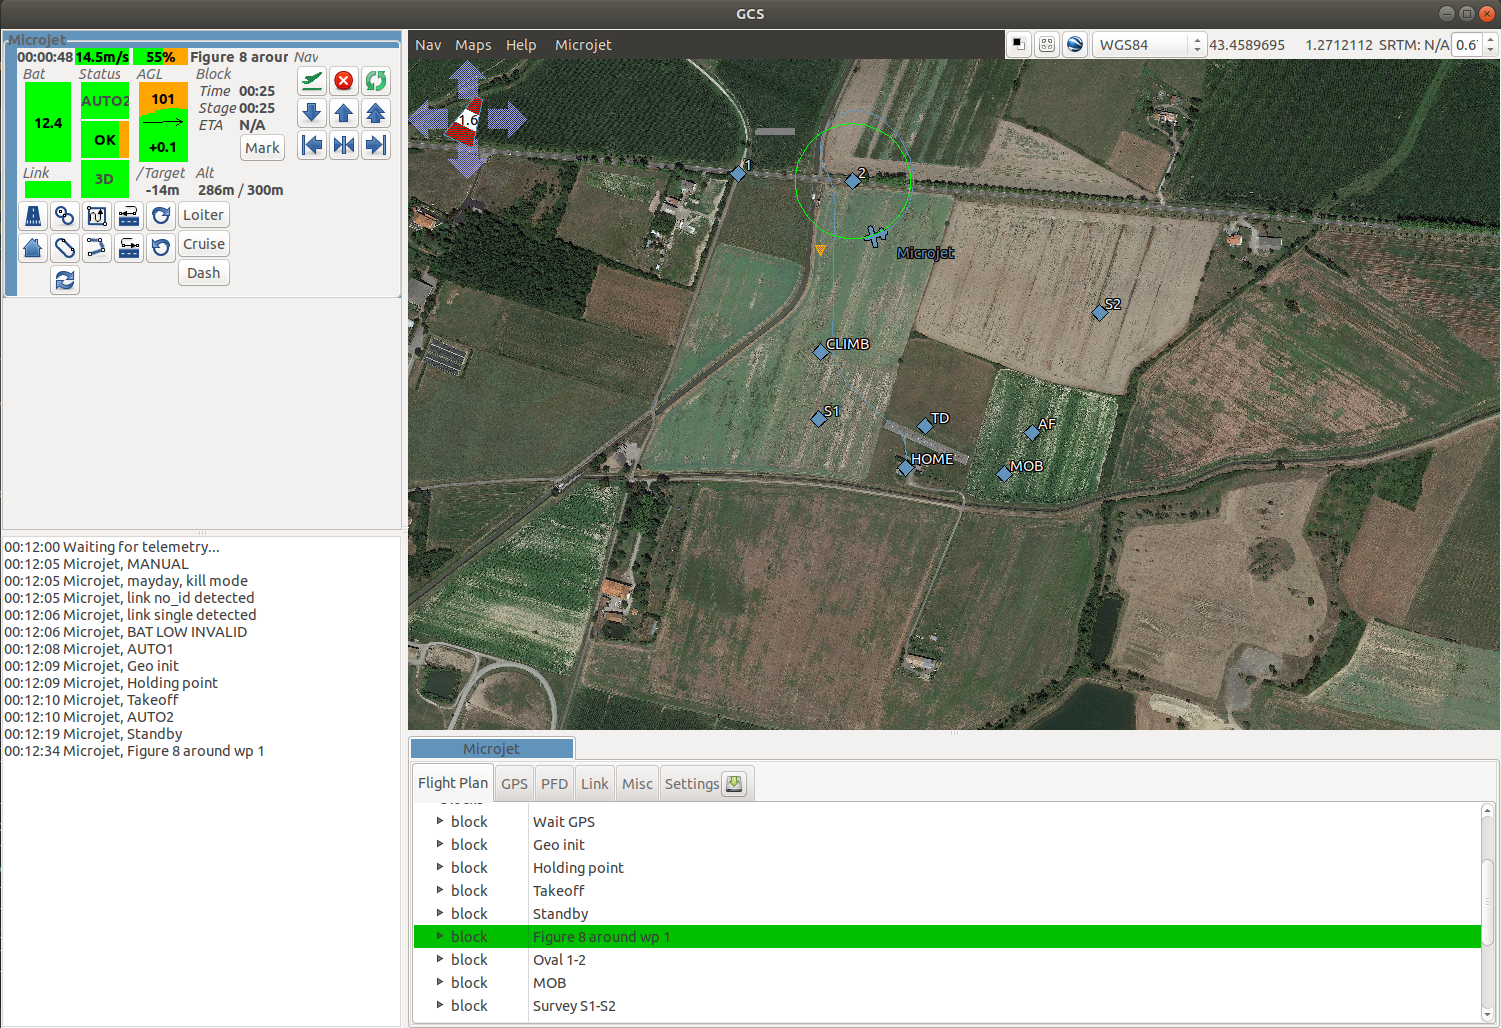
\includegraphics[width=\textwidth]{4_files/GCS.png}
    \caption{A snapshot of ground control station software (GCS), visualizing the map, waypoints (blue diamonds), the aircraft, its flight history (blue), the intended flight path (green), as well as its state (bottom in green) and some telemetry data (top left). The plan that it is following is one of the automatically generated test scenarios.}
    \label{fig:paparazzi_gcs}
\end{figure}

Test runner can move waypoints as well. The user can fix any number of waypoints at specified locations, providing their latitude longitude and altitudes. It can also randomize their location inside a cube. Boundaries of that cube (i.e. east-west, north-south, and floor-ceiling) are customizable through provided command line arguments.

The comprehensive list of command line arguments is included in Table~\ref{tab:test_runner_commandline_args} in \hyperref[appendixa]{Appendix~A}.


\subsubsection{Automated Test Generator}
The test generator component is a fuzz test generator specifically designed for Paparazzi. An auto pilot has plenty of parameters to change. Many of them need to remain unchanged. For example, changing aerodynamic and physical parameters of an air frame will make it behave incorrectly or even crash. A naïve algorithm might be tempted to only change these parameters to optimize a metric of ``bug''s per test. To comply with the constraints in input format and range and optimize test scenario diversity without having to have thousands of tests, I opted for developing a specialized automated test generator. 

This test generator is completely compatible with Paparazzi and designed with specific needs of an auto pilot in mind. It begins with loading and parsing the one fixed wing flight plan that comes with Paparazzi. It defines multiple actions (control blocks) available to a fixed wing aircraft. Two important components in the flight plan that are used are the waypoint names and locations, and available blocks. A test scenario is generated by taking the initial flight plan and fuzzing three parameters about it:
\begin{enumerate}
    \item Waypoint locations
    \item Sequence of actions 
    \item Action timing
\end{enumerate}

The test generator can be configured to fuzz all or some of them. \hl{I generated 31 tests with fuzzing the last two. Please note that the sequence of actions can have any length between 1 and the number of possible actions (5, in my case). Also for each sequence, $n!$ different permutations can be made that will result in very different outcomes. That makes the number of tests, $5!\times1+4!\times5+3!\times10+2!\times10+1!\times5=325$. Also note that these generated tests are made of unique blocks, in other words, a test scenario does not contain plans like ``Do A then B then A again'' while these plans are perfectly valid. In case one wants to have such plans they can write test plans manually.} \hl{to move}

The output is a python module that contains a subclass of \verb|PlanBase|, as expected by the automated test executor. These two work together seamlessly and the user can just use them in a plug-and-play manner without touching the code. Though, the generated code is designed to be effortlessly understandable and easily editable it even incorporates some auto-generated comments in the code.

The full table of command line arguments that test generator accepts is presented in Table~\ref{tab:test_generator_commandline_args} in \hyperref[appendixa]{Appendix~A}. To provide an example, the following command generates tests of length (number of actions) 2 for `Microjet' aircraft and writes it to the file \verb|l2.py| in the specified directory. It fuzzes the location (latitude, longitude, and altitude) of waypoint `S2' in the default cube, just overriding the altitude bounds in 200 to 220 meters, while the coordinates of `S1' are fixed. The initialization and landing stages which must be excluded from the test scenario are also specified. 
\begin{lstlisting}[language=bash]
gen_test.py --exclude "Wait GPS" "Geo init" "Holding 
point" Takeoff Standby "Land Right AF-TD" "Land Left 
AF-TD" land final flare --fuzz-wps S2 \
--wp-fuzz-bounds-alt 200 220 -w S1 43.4659053 1.27 300 \
--length 2 Microjet pprz_tester/generated_plans/l2.py
\end{lstlisting}
Some of the available actions and all the waypoints in this flight plan can be seen in Figure~\ref{fig:paparazzi_gcs}.













\section{Experiment Execution Environment} \label{sec:machines_config}
Training and evaluation of the deep learning model was done on a single node running Ubuntu 18.04 LTS (Linux 5.3.0) equipped with Intel Core i7-9700 CPU, 32 gigabytes of main memory, and 8 gigabytes of GPU memory on a NVIDIA GeForce RTX 2080 graphics card.
The code was implemented using keras on TensorFlow 2.0.

The baseline models could not fit on that machine, so two nodes on Compute Canada's Beluga cluster, one with 6 CPUs and 75GiB of memory and one with 16 CPUs and 64GiB of memory, were used to train and evaluate them.
